\section{Muhammad Fahmi}
\subsection{Pemahaman Teori}
\subsubsection{Soal No. 1}
\hfill \break
Apa itu fungsi library matplotlib
\hfill \break
Matplotlib adalah sebuah library dari Python yang bersifat 2D kemudian dapat menghasilkan plot berkualitas tinggi dalam berbagai format dan dapat digunakan pada banyak platform.
Matplotlib juga dapat digunakan sebagai pembuat grafik di berbagai platform, seperti Python dan Jupyter. Grafik yang dapat dibuat bervariasi, contohnya ialah garis, batang, lingkaran, histogram, dll.

\subsubsection{Soal No. 2}
\hfill \break
Jelaskan langkah-langkah membuat sumbu X dan Y di matplotlib

\begin{enumerate}
	\item Langkah yang pertama ialah kita harus import library Matplotlib.	
	\lstinputlisting[firstline=2, lastline=2]{src/6/1174021/1174021.py}
	
	\item Langkah yang kedua ialah dengan membuat variabel x yang menampung list untuk digunakan pada sumbu x dan sebaliknya juga membuat variabel y yang menampung list untuk sumbu y.	
	\lstinputlisting[firstline=4, lastline=5]{src/6/1174021/1174021.py}
	
	\item Langkah yang ketiga ialah dengan memanggil fungsi plot dan isi parameter pertama dengan variabel x dan parameter kedua dengan variabel y.
	\lstinputlisting[firstline=7, lastline=7]{src/6/1174021/1174021.py}	

	\item Langkah yang terakhir yaitu dengan memanggil plot tadi dengan cara memanggil fungsi show.
	\lstinputlisting[firstline=9, lastline=9]{src/6/1174021/1174021.py}
	
\end{enumerate}
\hfill \break
\textbf{Adapun kode program keseluruhan pada contoh diatas ialah :}

\lstinputlisting[caption = Soal No.2, firstline=2, lastline=9]{src/6/1174021/1174021.py}

\hfill \break
\textbf{Hasil Compile}

\begin{figure}[H]
	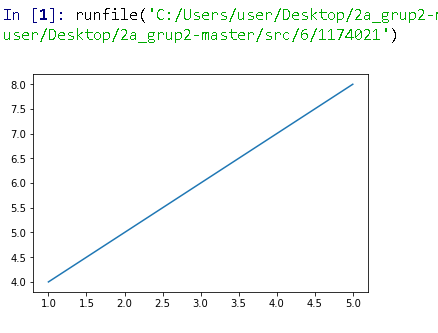
\includegraphics{figures/6/1174021/2.png}
	\centering
	\caption{Hasil compile Soal No.2}
\end{figure}
 
\subsubsection{Soal No. 3}
\hfill \break
Jelaskan bagaimana perbedaan fungsi dan cara pakai untuk berbagai jenis(bar, histogram ,scatter ,line, dll) jenis plot di matplotlib.

\begin{enumerate}
	\item \textbf{Bar Graph}
	
	Perbedaan bar graph dengan jenis plot yang lain ialah bar graph mempunyai tampilan seperti bar atau batang-batang yang berfungsi untuk membandingkan data untuk keperluan suatu hal.
	
	\textbf{Kode program bar graph}
	
	\lstinputlisting[caption = Soal No.3, firstline=13, lastline=25]{src/6/1174021/1174021.py}
	
	\textbf{Hasil Compile}
	
	\begin{figure}[H]
		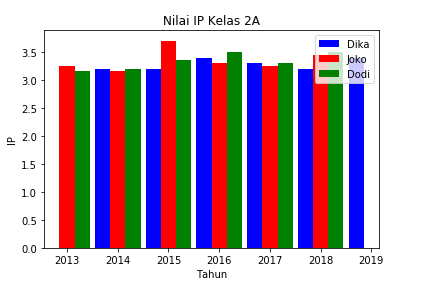
\includegraphics{figures/6/1174021/3.png}
		\centering
		\caption{Hasil compile bar graph}
	\end{figure}
	
	\item \textbf{Histogram}
	
	Perbedaan histogram dengan jenis plot yang lainnya ialah histogram menggunakan plot dimana plot yang dimunculkan adalah merupakan gabungan dari beberapa data yang telah dikelompokkan menjadi satu.
	
	\textbf{Kode Program histogram}
	
	\lstinputlisting[caption = Kode program histogram, firstline=29, lastline=36]{src/6/1174021/1174021.py}
	
	\textbf{Hasil Compile}
	
	\begin{figure}[H]
		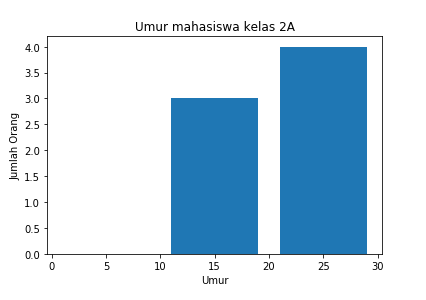
\includegraphics[width=12cm]{figures/6/1174021/31.png}
		\centering
		\caption{Hasil compile histogram}
	\end{figure}
	
	\item \textbf{Scatter Plot}
	
	Perbedaan scatter plot dengan jenis plot lain ialah scatter plot menggunakan tampilan data sebagai kumpulan titik dan masing-masing memiliki variabel untuk menentukan posisi pada sumbu horizontal dan sumbu vertikal.
	
	\textbf{Kode Program Scatter Plot}
	
	\lstinputlisting[caption = Kode program scatter plot, firstline=40, lastline=53]{src/6/1174021/1174021.py}
	
	\textbf{Hasil compile scatter plot}
	
	\begin{figure}[H]
		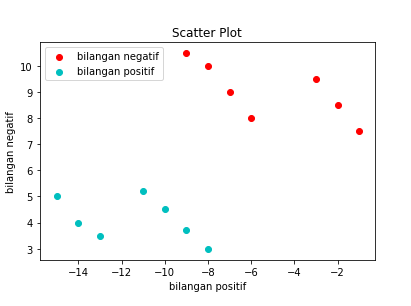
\includegraphics{figures/6/1174021/32.png}
		\centering
		\caption{Hasil compile membuat scatter plot menggunakan Matplotlib.}
	\end{figure}
	
	\item \textbf{Area Plot}
	
	Perbedaan area plot dengan jenis plot lain adalah area plot biasa digunakan untuk melakukan pelacakan perubahan dari waktu ke waktu untuk dua atau lebih kelompok terkait yang membentuk satu kategori secara keseluruhan.
	
	\textbf{Kode Program area plot}
	
	\lstinputlisting[caption = Kode program area plot, firstline=57, lastline=76]{src/6/1174021/1174021.py}
	
	\textbf{Hasil Compile area plot}
	
	\begin{figure}[H]
		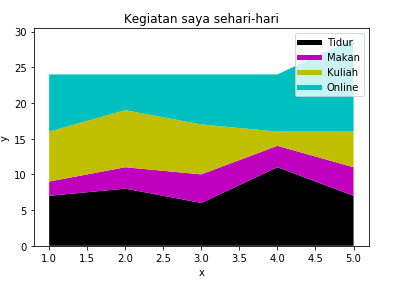
\includegraphics{figures/6/1174021/33.png}
		\centering
		\caption{Hasil compile area plot}
	\end{figure}
	
	\item \textbf{Pie Plot}
	
	Perbedaan pie plot dengan jenis plot lain ialah di pie plot kita menggunakan persentase atau data proporsional di mana setiap potongan pie mewakili kategori.
	
	\textbf{Kode Program pie plot}
	
	\lstinputlisting[caption = Kode program pie plot, firstline=80, lastline=101]{src/6/1174021/1174021.py}
	
	\textbf{Hasil Compile pie plot}
	
	\begin{figure}[H]
		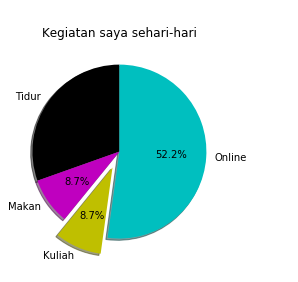
\includegraphics[width=9cm]{figures/6/1174021/34.png}
		\centering
		\caption{Hasil compile pie plot}
	\end{figure}
	
	\item \textbf{Line Graph}
	
	Perbedaan line graph dengan jenis plot lainnya ialah line graph menampilkan diagram dalam bentuk garis.
	
	\textbf{Kode Program line graph}
	
	\lstinputlisting[caption = Kode program line graph, firstline=105, lastline=113]{src/6/1174021/1174021.py}
	
	\textbf{Hasil Compile line graph}
	
	\begin{figure}[H]
		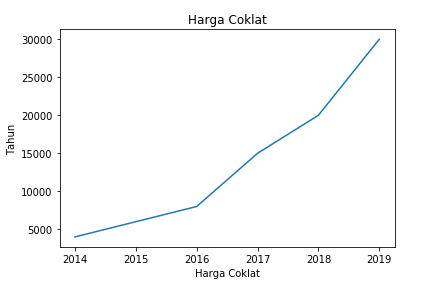
\includegraphics{figures/6/1174021/35.png}
		\centering
		\caption{Hasil compile line graph}
	\end{figure}
	
\end{enumerate}

\subsubsection{Soal No. 4}
\hfill \break
Jelaskan bagaimana cara menggunakan legend dan label serta kaitannya dengan fungsi tersebut.

\begin{enumerate}
	\item Untuk menggunakan legend, kita harus mendefinisikan setiap parameter label di tiap fungsi plot. Parameter label ini kemudian digunakan untuk memberikan label pada line sebagai pembeda antar line.
	
	\lstinputlisting[firstline=123, lastline=124]{src/6/1174021/1174021.py}
	
	\item Kemudian panggil fungsi legend.
	
	\lstinputlisting[firstline=128, lastline=128]{src/6/1174021/1174021.py}
\end{enumerate}

\hfill \break
\textbf{Kode Program Soal No.4}

\lstinputlisting[caption = Kode program Soal No.4, firstline=117, lastline=130]{src/6/1174021/1174021.py}

\hfill \break
\textbf{Hasil Compile soal no.4}

\begin{figure}[H]
	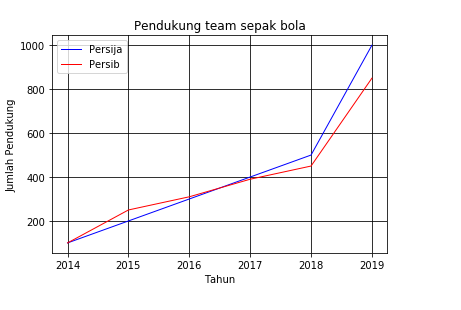
\includegraphics{figures/6/1174021/4.png}
	\centering
	\caption{Hasil compile soal no.4}
\end{figure}

\subsubsection{Soal No. 5}
\hfill \break
Jelaskan apa fungsi dari subplot di matplotlib, dan bagaimana cara kerja dari fungsi subplot, sertakan ilustrasi dan gambar sendiri dan apa parameternya jika ingin menggambar plot dengan 9 subplot di dalamnya.

\hfill \break
Fungsi subplot adalah untuk membuat beberapa plot di dalam satu gambar.
\hfill \break
Cara kerja subplot, yaitu fungsi subplot memiliki parameter pertama adalah jumlah kolom, parameter kedua adalah jumlah baris, dan parameter ketiga adalah index plot keberapanya.

\hfill \break
\textbf{Kode Program soal no.5}

\lstinputlisting[caption = Kode program membuat subplot menggunakan Matplotlib., firstline=134, lastline=146]{src/6/1174021/1174021.py}

\hfill \break
\textbf{Hasil Compile soal no.5}

\begin{figure}[H]
	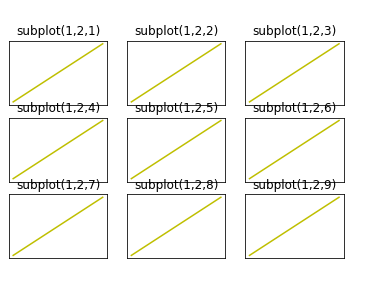
\includegraphics{figures/6/1174021/5.png}
	\centering
	\caption{Hasil compile soal no.5}
\end{figure}

\subsubsection{Soal No. 6}
\hfill \break
Sebutkan semua parameter color yang bisa digunakan (contoh:  m,c,r,k,...  dkk).

\begin{itemize}
	\item 'b' adalah kode untuk (blue)
	\item 'g' adalah kode untuk (green)
	\item 'r' adalah kode untuk (red)
	\item 'c' adalah kode untuk (cyan)
	\item 'm' adalah kode untuk (magenta)
	\item 'y' adalah kode untuk (yellow)
	\item 'k' adalah kode untuk (black)
	\item 'w' adalah kode untuk (white)
\end{itemize}

\subsubsection{Soal No. 7}
\hfill \break
Jelaskan bagaimana cara kerja dari fungsi hist, sertakan ilustrasi dan gambar sendiri.

\hfill \break
Cara kerja dari fungsi hist yaitu untuk menerima parameter yang telah diberikan, kemudian fungsi hist akan dieksekusi sesuai dengan parameter yang diberikan.

\hfill \break
\textbf{Kode Program soal no.7}

\lstinputlisting[caption = Kode program soal no.7, firstline=150, lastline=157]{src/6/1174021/1174021.py}

\hfill \break
\textbf{Hasil Compile soal no.7}

\begin{figure}[H]
	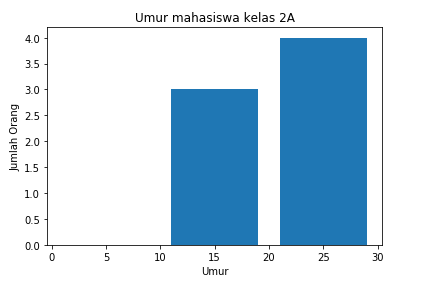
\includegraphics{figures/6/1174021/7.png}
	\centering
	\caption{Hasil compile soal no.7}
\end{figure}

\subsubsection{Soal No. 8}
\hfill \break
 Jelaskan lebih mendalam tentang parameter dari fungsi pie diantaranya labels, colors, startangle, shadow, explode, autopct.
 
 \begin{itemize}
 	\item labels digunakan untuk memberikan label di tiap persentase.
 	\item colors digunakan untuk memberikan warna di tiap persentase.
 	\item startangle digunakan untuk memutar plot sesuai dengan derajat yang ditentukan.
 	\item shadow digunakan untuk memberikan bayangan pada plot.
 	\item explode digunakan untuk memisahkan antar tiap potongan pie pada plot.
 	\item autopct digunakan untuk menentukan jumlah angka dibelakang koma.
 \end{itemize}
 
 